\documentclass[journal,10pt,twocolumn]{article}
\usepackage{graphicx, float}
\usepackage[margin=0.5in]{geometry}
\usepackage{amsmath, bm}
\usepackage{array}
\usepackage{booktabs}

\providecommand{\norm}[1]{\left\lVert#1\right\rVert}
\let\vec\mathbf
\newcommand{\myvec}[1]{\ensuremath{\begin{pmatrix}#1\end{pmatrix}}}
\newcommand{\mydet}[1]{\ensuremath{\begin{vmatrix}#1\end{vmatrix}}}

\title{\textbf{Line Assignment}}
\author{Pallavarapu Sravan kumar}
\date{September 2022}

\begin{document}

\maketitle
\paragraph{\textit{\large Problem Statement} - Let PS be the median of the triangle with vertices P(2, 2), Q(6,-1) and R(7, 3). The equation of the line passing through (1,-1) and parallel to PS is :}
\section*{\large Solution}
\begin{figure}[H]
\centering
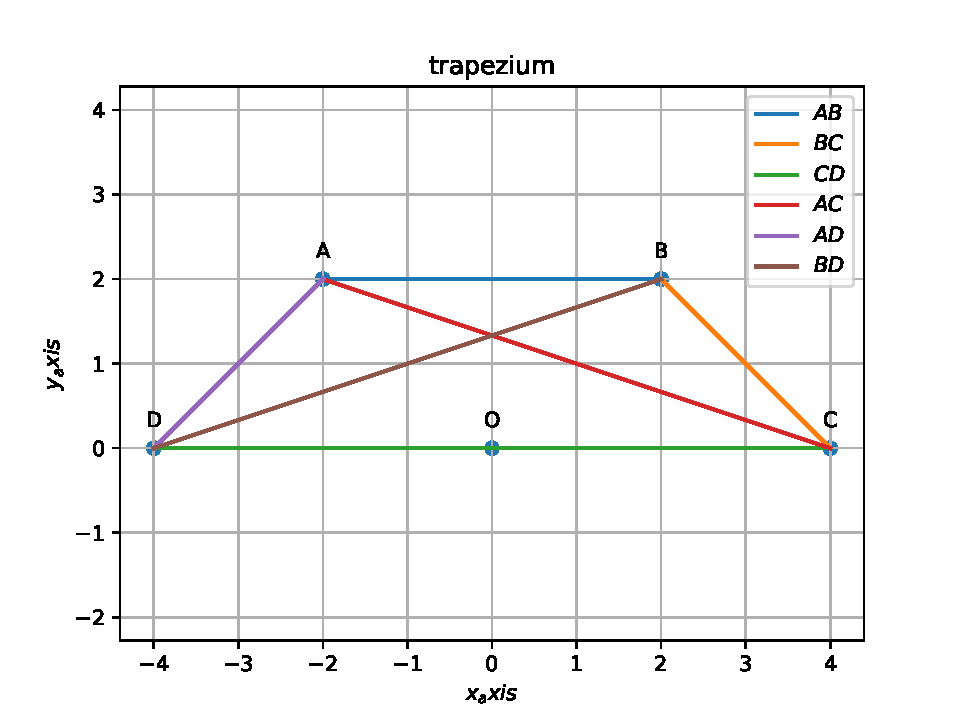
\includegraphics[width=1\columnwidth]{linefig.pdf}
\caption{}
\end{figure}

\section*{\large Construction}



The input parameters of figure 



\begin{table}[htbp]
 \begin{center}
    \begin{tabular}{|l|c|c|c|c|c|c} \hline \textbf{Symbol}
  & \textbf{value} & \textbf{Description} \\
 \hline
P &(2,2) & Point P in $\Delta$PQR\\ \hline
Q&(6,-1) & Point Q in $\Delta$PQR \\ \hline
R&(7,3)   & Point R in $\Delta$PQR\\ \hline
S&(13/2,1)   & median  of $\Delta$PQR\\ \hline
A&(1,-1)   & Point on the line equation\\ \hline
	
\end{tabular}   
\end{center}
\caption{\label{table:dummytable} }
\end{table}

\vspace*{10mm}


\section*{Proof:}

Given vector points of $\Delta$PQR 
\begin{eqnarray}
	\vec{P} = \myvec{2\\2},
	\vec{Q} = \myvec{6\\-1},
	\vec{R} = \myvec{7\\3}
\end{eqnarray}

PS is the median of $\Delta$PQR . So $\vec{S}$ is the midpoint between vector points $\vec{Q}$ and $\vec{R}$ .

\begin{eqnarray*}
	\vec{S}=\frac{\vec{Q}+\vec{R}}{2}	
    \end{eqnarray*}
\begin{eqnarray*}
	\vec{S}=\frac{\myvec{6\\-1}+\myvec{7\\3}}{2}
\end{eqnarray*}
\begin{eqnarray}
	\vec{S}=\myvec{6.5 \\1}
\end{eqnarray}
Directional vector $\vec{m}$  between vector points $\vec{P}$ and $\vec{S}$

\begin{eqnarray*}
	\vec{m}=\vec{S} - \vec{P}
\end{eqnarray*}

\begin{eqnarray*}
	\vec{m}=\myvec{6.5\\1} - \myvec{2 \\2}
\end{eqnarray*}


\begin{eqnarray}
	\vec{m}=\myvec{4.5\\-1}
\end{eqnarray}



Normal vector of this directional vector is
\begin{eqnarray}
\vec{n} = 	\myvec{1\\4.5}
\end{eqnarray}

The required line is parallel to vector $\vec{PS}$ and passes through the vector point $\vec{A}$ = $\myvec{1\\-1}$

\begin{eqnarray*}
\vec{n^T}\vec{(X-P)} = 0	
\end{eqnarray*}

\begin{eqnarray*}
	\myvec{1 \ 4.5}\myvec{\myvec{x\\y}-\myvec{1\\-1}}=0
\end{eqnarray*}

\begin{eqnarray}
        \myvec{1 \ 4.5}\myvec{x\\y}=-3.5
\end{eqnarray}




\end{document}
